\documentclass[english,8pt, a4paper]{amsart}
%\usepackage[english,norsk]{babel}
\usepackage[english]{babel}
\usepackage[utf8]{inputenc}
\usepackage[left=25mm, right=25mm]{geometry}
 
\usepackage{geometry}   % Margins
\usepackage{graphicx}   % Images
\usepackage{float}      % Image floating
%\usepackage{siunitx}    % SI-units
\usepackage{amsmath}
\DeclareMathOperator*{\argmin}{argmin}
\usepackage{verbatim}
\usepackage{url}
\usepackage{hyperref}
\usepackage{listings}
\usepackage{framed}
\usepackage{physics}
\usepackage[]{algorithm2e}
\numberwithin{figure}{section}
\numberwithin{table}{section}
\bibliographystyle{plain}

\SetKwFor{For}{for (}{) $\lbrace$}{$\rbrace$}
\newcommand{\bs}[1]{\boldsymbol{#1}}

\usepackage{color}
%\usepackage{multicol}
%\setlength\columnsep{14pt}
 
\definecolor{codegreen}{RGB}{0, 146, 146}
\definecolor{codegray}{rgb}{0.4,0.4,0.4}
\definecolor{codeblue}{RGB}{0, 109, 219}
\definecolor{backcolour}{rgb}{0.9,0.9,0.9}
 
\lstdefinestyle{mystyle}{
    backgroundcolor=\color{backcolour},
    commentstyle=\color{codegreen},
    keywordstyle=\color{magenta},
    numberstyle=\tiny\color{codegray},
    stringstyle=\color{codeblue},
    basicstyle=\footnotesize,
    breakatwhitespace=false,
    showstringspaces=false,
    breaklines=true,
    captionpos=b,
    keepspaces=true,
    numbers=left,
    numbersep=5pt,
    showspaces=false,
    basicstyle=\footnotesize \ttfamily \color{black} \bfseries,
    xleftmargin=0.4cm,
    frame=tlbr, framesep=0.1cm, framerule=0pt,
    showtabs=false,
    tabsize=2
}

%---------- included files ------------------------
\includeonly
{
    Sections/Introduksjon,
    Sections/Teori, 
    Sections/Eksperimentelt,
    Sections/Resultater,
    Sections/Diskusjon,
    Sections/Konklusjon,
    %Sections/Future,
}
 
\lstset{style=mystyle}
 
 
\title[Regression Analysis and Resampling Methods]{\large FYS-STK4155 - Project 1: \\
Regression Analysis and Resampling Methods}
\author[Sexton, Husom]{Alexander Harold Sexton \\ Erik Johannes Husom \\ \\ \today}
 
 
\begin{document}

\maketitle
\begin{abstract}
 
In this project we apply the Ordinary Least Squares method, Ridge regression and Lasso regression, in combination with the Bootstrap resampling technique, on two different data sets: Data generated from the Franke function and a topographical terrain data set. We compared the three different regression methods, and the OLS method gave us the lowest means squared error on test data in both cases, with respectively $\text{MSE}_{\text{Franke}}=0.0136$ and $\text{MSE}_{\text{terrain}}=0.0091$. 






%Even though the Ridge and Lasso regression produced a higher MSE, this might have been the result of lack of proper normalization of the data. 

%The Ridge regression gave only slightly worse results, with $\text{MSE}_{\text{Franke}}=0.0139$ and $\text{MSE}_{\text{terrain}}=0.0092$

%When creating a model for the terrain data, we
 
 
\end{abstract}
 
\tableofcontents
 
%\begin{multicols}{2}
\section{Introduction}\label{sec:Introduction}

Regression methods are a set of commonly used tools in machine learning, and the overarching goal is to study the dependence of a target or response variable on a number of independent variables, often called predictors. In order to perform regression we need a data set that contains information about the phenomenon we want to study, and this is used to estimate a function $f$, which is assumed to represent the relationship between the predictors and the response. The result is a model which can be used to understand how the response variable is related to the input variables, or just simply to predict the outcome based on new input data.

The aim of this project is to analyze different regression methods, specifically the Ordinary Least Squares (OLS) method, Ridge regression and Lasso regression. The OLS is one the most common approaches when performing linear regression, and produces a set of polynomial coefficients that describe the model as a function. Ridge and Lasso regression are two types of shrinkage methods that, in contrast to OLS, may reduce or "shrink" some of the coefficients in the model, which may be desirable if some predictors are more important than others, or if some of the predictors in a data set are correlated.

Another important aspect of this project is to explore resampling of data. We have specifically looked at the resampling technique called \textit{bootstrap}, where we draw random samples from a training data set multiple times, and refit a model with each of the samples. By doing this we can extract additional information about the data set.

In the first part of this project, we used a generated data set based on a function called the Franke function, and analyzed the performance of our chosen regression methods, including resampling of the data. In the second and last part, we applied the same techniques on topographical terrain data from an area of Norway.

This report includes the theory used in the project, along with a short review of the methods we implemented in our source code. Then we present our results, followed by a discussion, and lastly a conclusion where we sum up the most important findings.
\section{Theory}\label{sec:Theory}

\subsection{Ordinary Least Squares}
Suppose we have a collection of data consisting of a set of observations $\textbf{y} = [y_0, y_1, .., y_{n-1}]$, which are assumed to be the response of a set of variables $\textbf{x} = [x_0, x_1, .., x_{n-1}]$, described by some unknown function $f$. With no underlying knowledge of $f$, and a motivation to predict values of $y$ which are not in the original data set, it is usual to assume that there is a linear relationship between $\textbf{x}$ and $\textbf{y}$. A parameterization of $f$ can be chosen based upon some insight of the behaviour of $\textbf{y}$ wrt. $\textbf{x}$, and in the simplest case a polynomial of degree $p$, that is 
\begin{align}
    \label{eq:linearModel}
    y = y(x) \rightarrow y(x_i) = \Tilde{y}_i + \epsilon_i = \sum_{j=0}^{p}\beta_jx_i^j + \epsilon_i
\end{align}
where $\beta_j$ is an unknown parameter and $\epsilon_i$ is the error in our prediction $y_i$, which accounts for influences on our prediction values from other sources than our predictors $x_i$. This gives rise to the set of equations
\begin{align*}
    y_0&=\beta_0+\beta_1x_0^1+\beta_2x_0^2+\dots+\beta_{n-1}x_0^{p}+\epsilon_0\\
    y_1&=\beta_0+\beta_1x_1^1+\beta_2x_1^2+\dots+\beta_{n-1}x_1^{p}+\epsilon_1\\
    y_2&=\beta_0+\beta_1x_2^1+\beta_2x_2^2+\dots+\beta_{n-1}x_2^{p}+\epsilon_2\\
    &\vdots \\
    y_{n-1}&=\beta_0+\beta_1x_{n-1}^1+\beta_2x_{n-1}^2+\dots+\beta_{n-1}x_{p}^{n-1}+\epsilon_{n-1}
\end{align*}
We can rewrite this as a linear algebra problem by defining the vectors
\begin{align*}
    &\textbf{y} = [y_0,y_1, y_2,..., y_{n-1}]^T\\
    &\boldsymbol{\beta} = [\beta_0,\beta_1, \beta_2,\dots, \beta_{p}]^T\\
    &\boldsymbol{\epsilon} = [\epsilon_0,\epsilon_1, \epsilon_2,\dots, \epsilon_{n-1}]^T
\end{align*}
and the matrix 
\begin{align}
    \boldsymbol{X}=
    \begin{bmatrix} 
    1& x_{0}^1 &x_{0}^2& \dots &x_{0}^{p}\\
    1& x_{1}^1 &x_{1}^2& \dots &x_{1}^{p}\\
    1& x_{2}^1 &x_{2}^2& \dots &x_{2}^{p}\\                      
    \vdots& \vdots &\vdots& \cdots &\vdots\\
    1& x_{n-1}^1 &x_{n-1}^2& \dots &x_{n-1}^{p}\\
    \end{bmatrix}
    \label{eq:designmatrix}
\end{align}
where $\textbf{X} \in \mathbb{R}^{n \times p}$ is known as the \textit{design matrix}\footnote{In general, we are not restricted to a polynomial of only one variable. For a polynomial of degree $p$ with two variables, the design matrix would consist of every permutation of $x^i y^{p-i}$ along each row.}. Equation \ref{eq:linearModel} can then be written as
\begin{align}
    \boldsymbol{y} = \boldsymbol{\Tilde{y}} + \boldsymbol{\epsilon} = \boldsymbol{X\beta} + \boldsymbol{\epsilon}
    \label{eq:OLSmodel}
\end{align}
Ordinary Least Squares is a method of estimating the parameters $\boldsymbol{\beta}$, which minimizes the distance between our target $y_i$ and the prediction $\Tilde{y}_i$. A measure of this fit is the mean squared error \cite[p. 29]{james}
\begin{align}
    \label{eq:MSE}
    \text{MSE}(y_i, \Tilde{y}_i) =  \frac{1}{n} \sum_{i=0}^{n-1} (y_i - \Tilde{y}_i)^2
\end{align}
which we define as our \textit{cost function} 
\begin{align}
    C(\boldsymbol{\beta}) = \frac{1}{n}(\boldsymbol{y} - \boldsymbol{X\beta})^T(\boldsymbol{y} - \boldsymbol{X\beta})
\end{align}
Since this is a convex function of $\boldsymbol{\beta}$, it has a unique minimum which occurs when its gradient is equal to zero. By differentiating wrt. $\boldsymbol{\beta}$ and setting it equal to zero, we obtain
\begin{align}
    \pdv{C(\boldsymbol{\beta})}{\beta} &= -\frac{2}{n}\boldsymbol{X}^T(\boldsymbol{y} - \boldsymbol{X\beta}) = 0\\
    \boldsymbol{X}^T\boldsymbol{y} &= \boldsymbol{X}^T\boldsymbol{X\beta},
\end{align}
assuming that $\boldsymbol{X}^T\boldsymbol{X}$ is positive definite. This gives us the optimal values for the parameters $\boldsymbol{\beta}$:
\begin{align}
    \label{eq:betaoptols}
    \boldsymbol{\beta} = ( \boldsymbol{X}^T\boldsymbol{X})^{-1} \boldsymbol{X}^T \boldsymbol{y}
\end{align}
The predicted outputs $\boldsymbol{\Tilde{y}}$ for a given input $\boldsymbol{X}$ is then given by
\begin{align}
    \boldsymbol{\Tilde{y}} = \boldsymbol{X\beta} = \boldsymbol{X}(\boldsymbol{X}^T\boldsymbol{X})^{-1}\boldsymbol{X}^T
\end{align}
The predicted values $\boldsymbol{\tilde{y}}$ can be viewed as and orthogonal projection of $\boldsymbol{y}$ onto the vector space spanned by the columns of $\boldsymbol{X}$. The variance of the coefficients $\beta$ is

\begin{align}
    \text{Var} (\beta) &= \text{Var} \big((\boldsymbol{X}^T\boldsymbol{X})^{-1} \boldsymbol{X}^T \boldsymbol{y} \big) \\
    &= (\boldsymbol{X}^T\boldsymbol{X})^{-1} \bs{X}^T \text{Var} (\bs{y}) \big((\boldsymbol{X}^T\boldsymbol{X})^{-1} \bs{X}^T\big)^T\\
    &= \text{Var}(\bs{y})(\boldsymbol{X}^T\boldsymbol{X})^{-1}
\end{align}


\subsection{Ridge and Lasso Regression}

There are several ways we can try to improve the Ordinary Least Squares method. The coefficients produced by the OLS method may often have a low bias and a large variance (to be discussed in the following subsection), and it treats all parameters in the same way without taking into account that some predictors may be more important than others. We can improve the prediction accuracy by removing or reducing some of the coefficients, and Ridge regression is a method that shrinks the coefficients according to a penalty on their size. We introduce a \textit{tuning parameter} $\lambda \geq 0$, which quantifies the amount of shrinkage. For Ridge regression, our cost function is\cite[p. 64]{hastie}:
\begin{align}
    C(\boldsymbol{\beta}) = (\boldsymbol{y} - \boldsymbol{X\beta})^T(\boldsymbol{y} - \boldsymbol{X\beta}) + \lambda \boldsymbol{\beta}^T\boldsymbol{\beta}
\end{align}

By taking the derivatives wrt. $\boldsymbol{\beta}$, as we did with the Ordniary Least Squares method, we obtain that the optimal values for the parameters $\boldsymbol{\beta}$ are:
\begin{align}
    \label{eq:betaoptridge}
    \boldsymbol{\beta} = ( \boldsymbol{X}^T\boldsymbol{X} + \lambda \boldsymbol{I} )^{-1} \boldsymbol{X}^T \boldsymbol{y},
\end{align}
and the predicted outputs $\boldsymbol{\Tilde{y}}$ for a given  $\boldsymbol{X}$ is
\begin{align}
    \boldsymbol{\Tilde{y}} = \boldsymbol{X\beta} = \boldsymbol{X}(\boldsymbol{X}^T\boldsymbol{X}  + \lambda \boldsymbol{I})^{-1}\boldsymbol{X}^T
\end{align}

We can see that setting $\lambda=0$ results in the Ordinary Least Squares method.

Another shrinkage method is the Lasso (Least Absolute Shrinkage and Selection Operator) method, which uses the cost function\cite[p. 219]{james}
\begin{align}
    C(\boldsymbol{\beta}) = (\boldsymbol{y} - \boldsymbol{X\beta})^T(\boldsymbol{y} - \boldsymbol{X\beta}) + \lambda \sqrt{\boldsymbol{\beta}^T\boldsymbol{\beta}}
\end{align}

The difference between Ridge and Lasso regression is that we replace the $L_2$ ridge penalty $||\boldsymbol{\beta}||_2^2 = \boldsymbol{\beta}^T\boldsymbol{\beta}$ with the $L_1$ Lasso penalty $||\boldsymbol{\beta}||_1 = \sqrt{\boldsymbol{\beta}^T\boldsymbol{\beta}}$. This altered penalty means that the solutions in the $y_i$ becomes nonlinear, and we cannot find a closed form expression for the parameters. Instead, the Lasso method uses gradient descent to find the minimum of the function\footnote{The specific details of the theory behind the Lasso method and gradient descent algorithms is outside the scope of this project, which is also why we use the Python library Scikit Learn to perform this type of regression.}. When using the $L_1$ norm instead of the $L_2$ norm we may end up with some coefficients being set to zero.

The tuning parameter $\lambda$ needs to be selected carefully, and can be tuned by using for example cross-validation or Bootstrapping.

\subsection{Error analysis}

In order to evaluate the fit of the different models in this project, we use several indicators. One of the most common error measures is the \textit{mean squared error} (MSE), which is already defined in equation \ref{eq:MSE}. The MSE will be small if the predicted values are close to the true values, which is the ideal scenario.

Another measure is the $R^2$ score\cite[p. 70]{james}:

\begin{align}
    R^2 (y, \Tilde{y}) = 1 - \frac{\sum_{i=0}^{n-1}(y_i - \Tilde{y}_i)^2}{\sum_{i=0}^{n-1}(y_i - \Bar{y})^2},
\end{align}
where $\Bar{y}$ is

\begin{align}
    \Bar{y} = \frac{1}{n} \sum_{i=0}^{n-1} y_i.
\end{align}

The $R^2$ score tells us how much of the variance in the response variable that is explained by the model. The value is ideally between 0 and 1, and a number close to 1 generally indicates that there is a strong relationship between the input variables and the response.

\subsection{Bias-Variance Tradeoff}

Bias and variance are two important quantities when it comes to predictive models. The bias is a measure of the difference between our prediction and the true value that we want to predict. Models with high bias tends to underfit the data, i. e. the model is oversimplified. Variance is an indicator of how sensitive the machine learning method is to the specific training data set. A high variance means that the model tends to be very affected by small fluctuations and noise in the predictors, and this leads in an overfitted model. As mentioned above, the quality of fit of a model is often measured using the MSE, which should be minimized, and we will now show how the MSE can be decomposed into three parts: Bias, variance and irreducible error.

Variance is in general defined as
\begin{align}    
    \label{eq:var1}
    \text{Var}(x) &= \mathbb{E}\left[(x - \mathbb{E}[x])^2\right]\\
    &= \mathbb{E}[x^2] - \mathbb{E}[x]^2
    \label{eq:var2}
\end{align}



The bias of our prediction $\bs{\tilde{y}}$ can be mathematically written in the following way\cite[p. 24]{hastie}:

\begin{align}
    \text{Bias}(\boldsymbol{\tilde{y}}) &= \mathbb{E}[\boldsymbol{\tilde{y}} - f]\\
    &= \mathbb{E}[\boldsymbol{\tilde{y}}] - f
\end{align}
    

The MSE, which is also the basis of the cost function for the OLS method, is given as:
\begin{align}
    \text{MSE} = C(\boldsymbol{X},\boldsymbol{\beta}) =\frac{1}{n}\sum_{i=0}^{n-1}(y_i-\tilde{y}_i)^2=\mathbb{E}\left[(\boldsymbol{y}-\boldsymbol{\tilde{y}})^2\right].
    \label{eq:MSEbiasvar}
\end{align}

% By decomposing this expression we get:
% \begin{align}
%     \mathbb{E}\left[(\boldsymbol{y}-\boldsymbol{\tilde{y}})^2\right] &= \mathbb{E}\left[ \boldsymbol{\tilde{y}}^2 - 2\boldsymbol{\tilde{y}}\boldsymbol{y} + \boldsymbol{y}^2 \right]\\
%     &= \mathbb{E}\left[ \boldsymbol{\tilde{y}}^2 \right] - 2\mathbb{E}\left[ \boldsymbol{\tilde{y}} \right]\boldsymbol{y} + \boldsymbol{y}^2\\
%     &= \mathbb{E}\left[ \boldsymbol{\tilde{y}}^2 \right] - \mathbb{E}\left[ \boldsymbol{\tilde{y}} \right]^2 + \mathbb{E}\left[ \boldsymbol{\tilde{y}} \right]^2 - 2\mathbb{E}\left[ \boldsymbol{\tilde{y}} \right]\boldsymbol{y} + \boldsymbol{y}^2\\
%     &=  \mathbb{E}\left[(\boldsymbol{\tilde{y}} - \mathbb{E}[\boldsymbol{\tilde{y}}])^2\right] + \left(\mathbb{E}\left[ \boldsymbol{\tilde{y}} \right] - \boldsymbol{y} \right)^2\\
%     &=\frac{1}{n}\sum_i(\tilde{y}_i-\mathbb{E}\left[\boldsymbol{\tilde{y}}\right])^2 + \frac{1}{n}\sum_i(\mathbb{E}\left[\boldsymbol{\tilde{y}}\right] - y_i )^2 + \sigma^2 ,\\
%     &= \text{Var}(\boldsymbol{\tilde{y}}) + \text{Bias}(\boldsymbol{\tilde{y}})^2 + \text{Var}(\epsilon).
% \end{align}

We will assume that $\bs{y} = f(x) + \varepsilon$, where $\varepsilon$ is the noise with zero mean and a variance of $\sigma^2$. This means that $\mathbb{E}[\varepsilon] = 0$ and $\text{Var}(\varepsilon) = \sigma^2$. We also have that $\mathbb{E}[f] = f$ since $f$ is deterministic. Furthermore, the variance of $\bs{y}$ can be written as:

\begin{align}
    \text{Var}(\bs{y}) &= \mathbb{E}\left[(\boldsymbol{\tilde{y}} - \mathbb{E}[\boldsymbol{\tilde{y}}])^2\right]\\
    &= \mathbb{E}\big[(\bs{y} - f)^2\big] = \mathbb{E}\big[f + \varepsilon - f)^2\big]\\ 
    &= \mathbb{E}\big[\varepsilon^2\big]\\
    &= \text{Var}[\varepsilon] + \mathbb{E}[\varepsilon]^2 \\
    &= \sigma^2
\end{align}
In the last equality we use the rearranged version of equation \ref{eq:var2}: $\mathbb{E}[x^2] = \text{Var}(x) + \mathbb{E}[x]^2$. The information above can then be used to decompose the MSE from equation \ref{eq:MSEbiasvar}:

\begin{align}
    \mathbb {E} {\big [}(\bs{y} - {\bs{\tilde{y}}})^{2}{\big ]}&=\mathbb {E} {\big [}(f+\varepsilon -{\bs{\tilde{y}}})^{2}{\big ]}\\
    &=\mathbb {E} {\big [}(f+\varepsilon -{\bs{\tilde{y}}}+\mathbb {E} [{\bs{\tilde{y}}}]-\mathbb {E} [{\bs{\tilde{y}}}])^{2}{\big ]}\\
    &=\mathbb {E} {\big [}(f-\mathbb {E} [{\bs{\tilde{y}}}])^{2}{\big ]}+\mathbb {E} [\varepsilon ^{2}]+\mathbb {E} {\big [}(\mathbb {E} [{\bs{\tilde{y}}}]-{\bs{\tilde{y}}})^{2}{\big ]} \\ 
    &\hspace{0.5cm}+2\mathbb {E} {\big [}(f-\mathbb {E} [{\bs{\tilde{y}}}])\varepsilon {\big ]}+2\mathbb {E} {\big [}\varepsilon (\mathbb {E} [{\bs{\tilde{y}}}]-{\bs{\tilde{y}}}){\big ]}+2\mathbb {E} {\big [}(\mathbb {E} [{\bs{\tilde{y}}}]-{\bs{\tilde{y}}})(f-\mathbb {E} [{\bs{\tilde{y}}}]){\big ]}\\
    &=(f-\mathbb {E} [{\bs{\tilde{y}}}])^{2}+\mathbb {E} [\varepsilon ^{2}]+\mathbb {E} {\big [}(\mathbb {E} [{\bs{\tilde{y}}}]-{\bs{\tilde{y}}})^{2}{\big ]}+2(f-\mathbb {E} [{\bs{\tilde{y}}}])\mathbb {E} [\varepsilon ]\\
    &\hspace{0.5cm}+2\mathbb {E} [\varepsilon ]\mathbb {E} {\big [}\mathbb {E} [{\bs{\tilde{y}}}]-{\bs{\tilde{y}}}{\big ]}+2\mathbb {E} {\big [}\mathbb {E} [{\bs{\tilde{y}}}]-{\bs{\tilde{y}}}{\big ]}(f-\mathbb {E} [{\bs{\tilde{y}}}])\\
    &=(f-\mathbb {E} [{\bs{\tilde{y}}}])^{2}+\mathbb {E} [\varepsilon ^{2}]+\mathbb {E} {\big [}(\mathbb {E} [{\bs{\tilde{y}}}]-{\bs{\tilde{y}}})^{2}{\big ]}\\
    &=(f-\mathbb {E} [{\bs{\tilde{y}}}])^{2}+\operatorname \sigma^2 +\operatorname {Var} {\big (}{\bs{\tilde{y}}}{\big )}\\
    &=\operatorname {Bias} ({\bs{\tilde{y}}})^{2}+\sigma ^{2}+\operatorname {Var} {\big (}{\bs{\tilde{y}}}{\big )}
\end{align}


The decomposition above shows us that to minimize the total error, we need to have both low bias and low variance ($\sigma^2$ is the irreducible error), i. e. we want to have a model that captures the trends in the training data while also performing well on test data that have not been included in training. The problem is that when using methods that give low bias we usually end up with a high variance, and similarly, low-variance methods results in high bias. This is why we need to find the optimal balance between bias and variance when choosing what learning method to use.


\subsection{Resampling Methods}

In order to extract as much information from the data set as possible, we use resampling methods. The idea is to select subsets of the training data set repeatedly, and refitting a model each time. In this project we use a resampling method called the Bootstrap method. If we have a training data set $\boldsymbol{Z} = (z_1, z_2, \dots, z_N)$ with $z_i = (x_i, y_i)$, we start by drawing a random dataset of size $N$ (i.e. the same size as the original training set), but allow datapoints to be drawn several times (draw with replacement). Then we fit a model to this dataset with our chosen method, which in this project is different regression methods, and analyze the performance of the fit. We repeat this process $B$ times, each time drawing a new data set from the original datset.


\subsection{Franke Function}

In order to analyze the different regression algorithms we used a sum of exponentials that is commonly used when testing fitting methods, called the Franke Function\cite{franke}:

\begin{multline}
\label{eq:franke}
f(x,y) = \frac{3}{4}\exp{\left(-\frac{(9x-2)^2}{4} - \frac{(9y-2)^2}{4}\right)}+\frac{3}{4}\exp{\left(-\frac{(9x+1)^2}{49}- \frac{(9y+1)}{10}\right)} \\
+\frac{1}{2}\exp{\left(-\frac{(9x-7)^2}{4} - \frac{(9y-3)^2}{4}\right)} -\frac{1}{5}\exp{\left(-(9x-4)^2 - (9y-7)^2\right) }.
\end{multline}


\section{Methods}\label{sec:Methods}
\subsection{Formatting the data}\label{sec:data_format}
We have two sources of data, one is generated by the Frankie function (equation \ref{eq:franke}), and the other is real terrain data in the form of elevation maps. In both cases, the prediction parameters are the $x_1$ and $x_2$ coordinates of the domain, and the height $y$ is the output. For the Frankie data, we generate $n$ uniformly distributed values of $x_1, x_2 \in [0,1]$ and place them in a mesh grid.  We evaluate the function at each point in the grid, and add stochastic noise $\epsilon \in \mathcal{N}(0, \sigma^2)$ to each point.

In the case of the real terrain data\footnote{The original data file can be found at the website \url{https://earthexplorer.usgs.gov} with Entity ID: SRTM1N41W001V3}, this is simply imported as a \textit{.tif} file, giving the terrain height in meters, which is rescaled to be in units of kilometers. We also resize the image, such that only $1/16$th of the original image is used. The original image is of dimensions $3600 \times 1800$ organized in a 2D array, where we have select the $900$ first points in the $x_1$ and $x_2$ directions as our data set. Finally we slice every other point in this array, such that the final image is of dimension $450 \times 450$. This is done due to memory issues when operating on larger data sets.

We now initialize our design matrix by organizing the values of $x_1$ and $x_2$ according to equation \ref{eq:designmatrix}, such that each column consist of a unique combination of powers $x_1^i x_2^{p-i}$, $i = 0,1,\dots,p$, and each row containing unique combinations of $x_1$ and $x_2$ values. We now have $\boldsymbol{X} \in \mathbb{R}^{n^2 \times p}$. The $\boldsymbol{y}$ values in our data are flattened to a 1D array, resulting in our target vector $\boldsymbol{y} \in \mathbb{R}^{n^2 \times 1}$. 

Ideally one would want to normalize the data, which involves subtracting the mean of each column from the corresponding column in $\boldsymbol{X}$ and also dividing each column by its standard deviation. However, we have had varying results when trying to implement this, but have not viewed it as a big problem, as the values of the data generated by the Franke function is mostly in the region $y \in [0, 1]$, which is also the case of the terrain data after converting from meters to kilometers.

\subsection{Regression Methods}
The main class in our implementation which performs the regression methods is called \textit{RegressionMethods}, and is instantiated simply with a specification of the desired method, that is, either ordinary least squares, Ridge or Lasso. To train the model, the class has a method called \textit{fit}, which takes as arguments the training data $\boldsymbol{X}_{train}$, and calls upon the relevant regression method. The ordinary least squares method finds the optimal $\boldsymbol{\beta}^{OLS}$ values by equation \ref{eq:betaoptols}, and does this by using the Numpy library's matrix multiplication functionality and \textit{linalg.pinv} function for finding the inverse matrix\footnote{In cases where the inverse matrix does not exists, it instead computes the pseudo-inverse.}. In the same manner, it computes the optimal $\boldsymbol{\beta}^{Ridge}$ by solving equation \ref{eq:betaoptridge}. In this case, the class must also be instantiated with the desired penalty parameter $\lambda$. This is also the case when using the class' Ridge regression method. We have not implemented this method ourselves, but instead uses the functionality of Scikit Learn's \textit{Lasso} function. Any instance of the model can also predict a set of input parameters different from those it has been trained on, this is done by calling the \textit{predict} method with an input parameter $\boldsymbol{X}_{test}$, which calculates the matrix-vector multiplication of $\boldsymbol{X}_{test}\boldsymbol{\beta} = \boldsymbol{\Tilde{y}}$.

\subsection{Resampling}
Our resampling method of choice is Bootstrapping, which we have implemented such that it first splits our data into training and test data, then randomly selects points and fits the model to these selected points. When this process has been completed a desired number of times, it calculates the error metrics of the predictions on both the test and training data. Pseudo-code for the algorithm:
\begin{algorithm}[!h]
{Split the data $\boldsymbol{X}$ and $\boldsymbol{y}$ into training data and test data}\\
\For{$n_{bootstraps}$}{
    {Select $n_{train}$ random samples from the training data}\\
    {Train the model on $\boldsymbol{X}_{train}$}\\
    {Test the model on $\boldsymbol{X}_{test}$}\\
    {Save all predicted values $\boldsymbol{\Tilde{y}}$}\\
}
{Calculate mean MSE, $R^2$ score, bias$^2$ and variance}
\end{algorithm}

In order to find the optimal parameters which gives the best fit to our data, we have also implemented a function which performs the above algorithm for chosen model value ranges of $\lambda$ and polynomial degrees $d$, and uses the MSE as a measure for how well the particular model performs.

\subsection{Benchmarks}
We have constructed a test case, which tests the results of our implementations of OLS and Ridge against the predictions of Scikit learn's methods. The data which is used in the test is generated from the Franke function, with $100 \times 100$ points. We then calculate the mean squared error between the prediction on this data produced by our code and Scikit learn's. In both cases the difference in the predictions was to machine presicion.
\subsection{Source code}

The source code of this project is written in Python, and can be found in the GitHub repository at \url{https://github.com/alexahs/FYS-STK4155/tree/master/Project_1}. The repository consists of the following files:
\begin{itemize}
    \item RegressionMethods.py
    \item Resamplnig.py
    \item unitTests.py
    \item functions.py
    \item analysis.py
    \item main.py
\end{itemize}



\section{Results}\label{sec:Results}

\subsection{Regression on generated data}
The performance of the ordinary least squares fit to the data is shown for different model complexities in figure \ref{fig:ols_frankie_train_test_bias_variance} (left). The prediction on test data has a minimum mean squared error of $\text{MSE} = 0.0136$ and $R^2 = 0.819$ (not shown in the plot), which occurs when the model complexity is of degree $d=5$, while the prediction on the training data has no minimum and keeps declining for higher complexity. The plot to the right in the same figure shows again the mean squared error of the predictions on the test data, and also its decomposition into bias$^2$ and variance. 
\begin{figure}[!h]
    \centering
    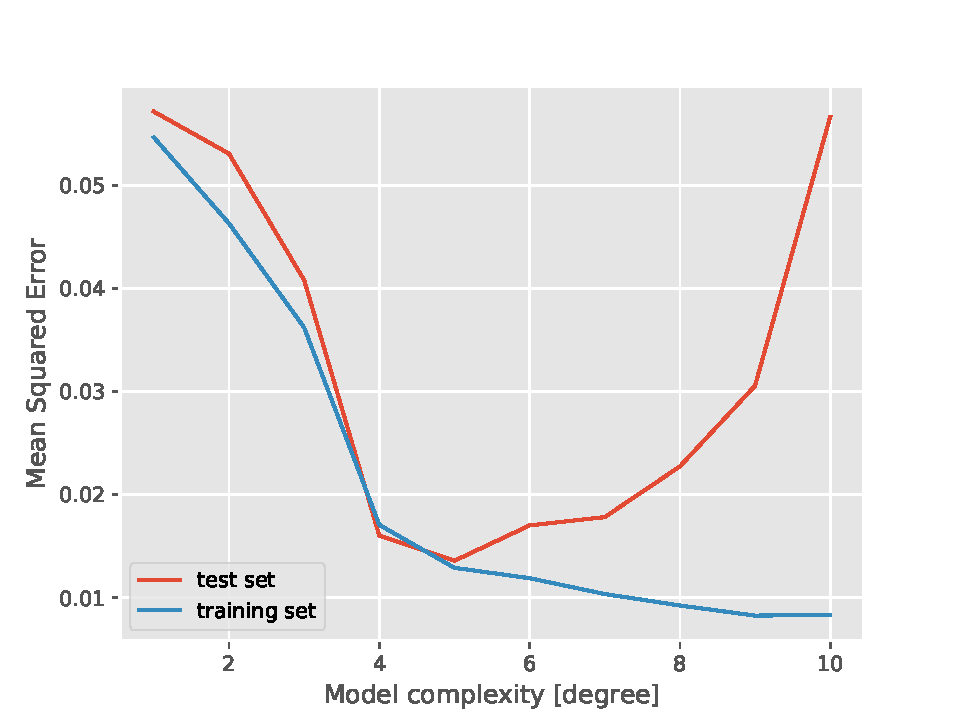
\includegraphics[scale=0.48]{Figures/OLS/deg_analysis_ols_test_train_001.pdf}
    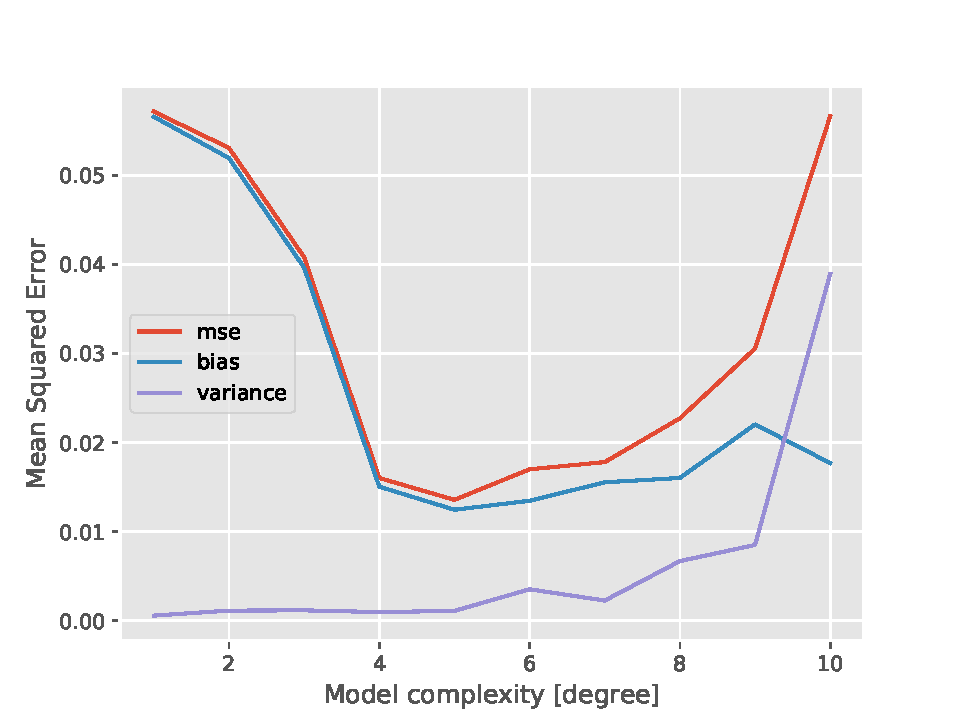
\includegraphics[scale=0.48]{Figures/OLS/deg_analysis_ols_bias_variance_002.pdf}
    \caption{Error in the OLS regression prediction on the generated data as a function of the models polynomial degree for the training and testing data (left). Figure to the right shows the bias$^2$ and variance decomposition of the MSE in the prediction on the test data.}
    \label{fig:ols_frankie_train_test_bias_variance}
\end{figure}
Figure \ref{fig:ols_frankie_confidence} also shows the confidence intervals of the different $\beta$ parameters for the optimal model with $d=5$.

For Ridge regression, figure \ref{fig:ridge_heatmap_frankie} shows the mean squared errors in the predictions on the test data for values of the hyper parameter $\lambda$ and polynomial degree $d$. The minimum error is at $\lambda = 10^{-4}$ and $d = 9$, with $\text{MSE} = 0.0139$\footnote{In the plot we see that the MSE is truncated at $0.013$, but an inspection of the data showed that the actual value was $0.0139$.} and $R^2 = 0.874$.
\begin{figure}[!h]
    \centering
    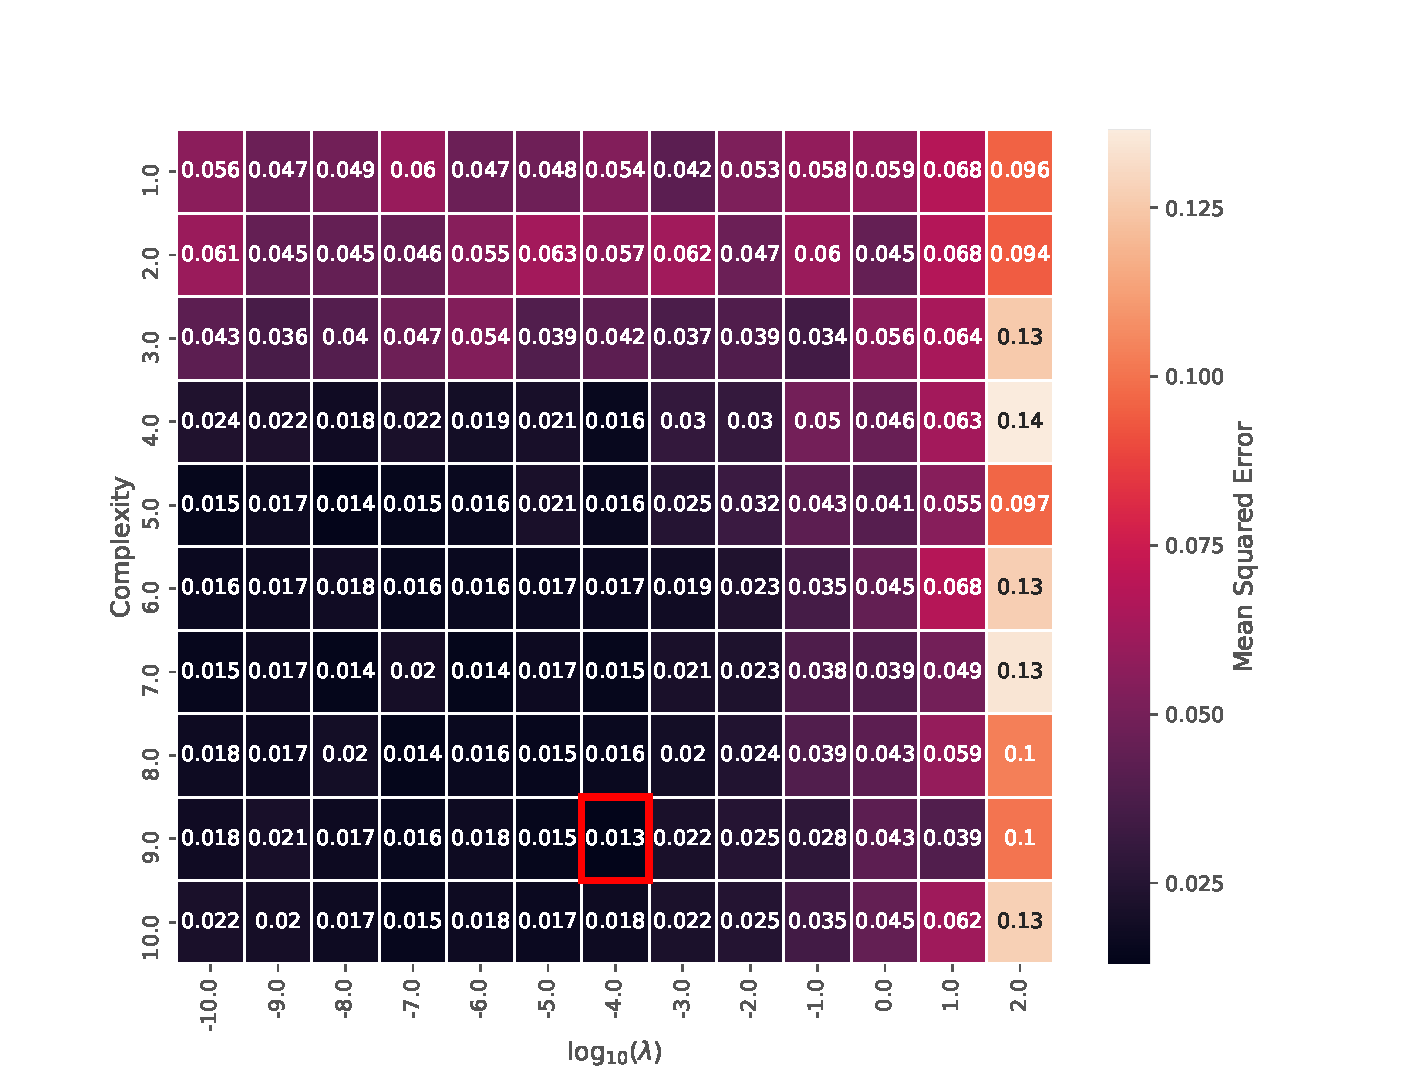
\includegraphics[scale=0.6]{Figures/RIDGE/min_mse_heatmap_ridge_003.pdf}
    \caption{Heat map of the MSE of the predictions of Ridge regression on the generated data for different values of $\lambda$ and model complexity $d$.}
    \label{fig:ridge_heatmap_frankie}
\end{figure}
\begin{figure}[!h]
    \centering
    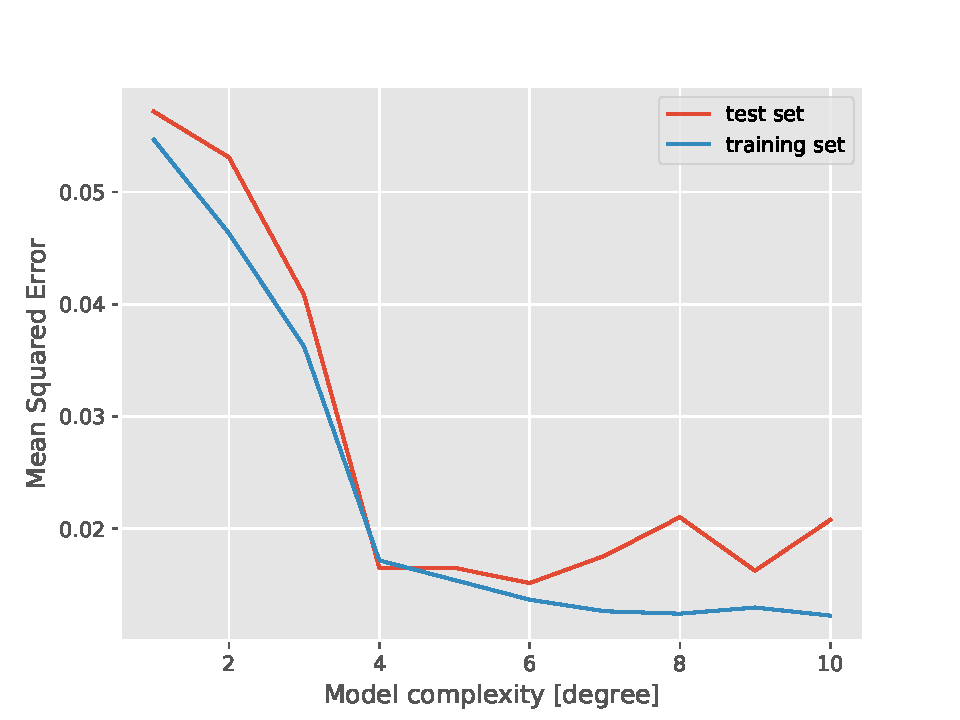
\includegraphics[scale=0.48]{Figures/RIDGE/deg_analysis_ridge_test_train_004.pdf}
    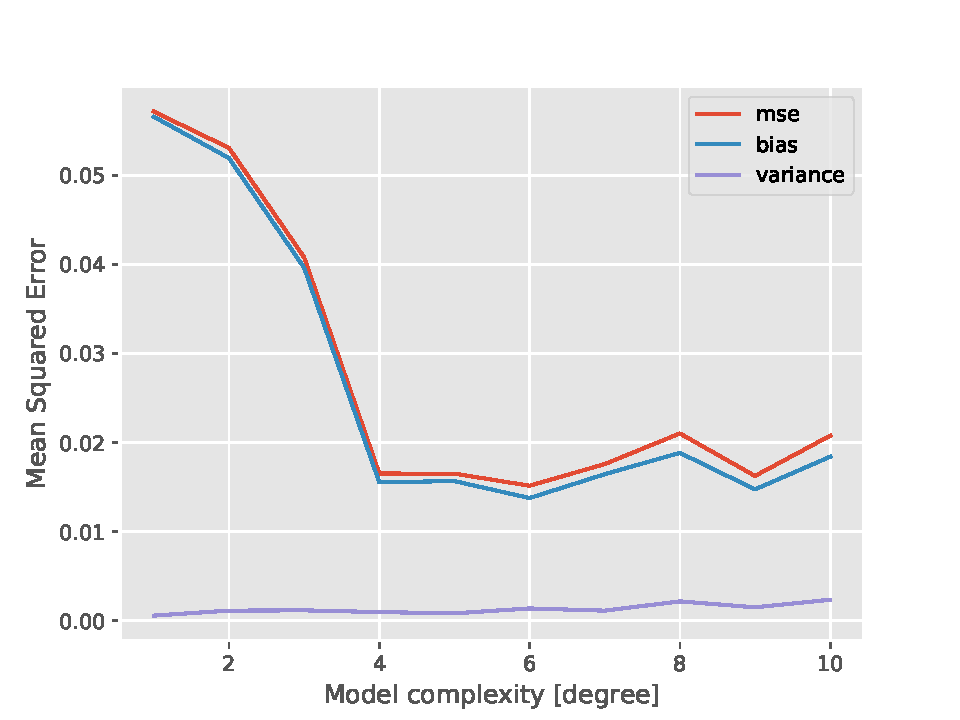
\includegraphics[scale=0.48]{Figures/RIDGE/deg_analysis_ridge_bias_variance_005.pdf}
    \caption{Error in the Ridge regression prediction on the generated data as a function of complexity, with $\lambda = 10^{-4}$. The left plot shows the error in the prediction on both the training and test data. The right plot shows the bias$^2$ and variance decomposition of the MSE on the test data.}
    \label{fig:ridge_frankie_train_test_bias_variance}
\end{figure}
Figure \ref{fig:ridge_frankie_train_test_bias_variance} shows the performance of Ridge regression in a separate run for different polynomial orders $d$, with the optimal value of $\lambda = 10^{-4}$ found in the above figure (\ref{fig:ridge_heatmap_frankie}). The figure shows the errors in both predictions on the test data and training data, as well as the bias$^2$ and variance decomposition of the error. Here we found the minimum predicted MSE to occur at $d = 6$, with $\text{MSE} = 0.151$ and $R^2 = 0.877$.


\begin{figure}[!h]
    \centering
    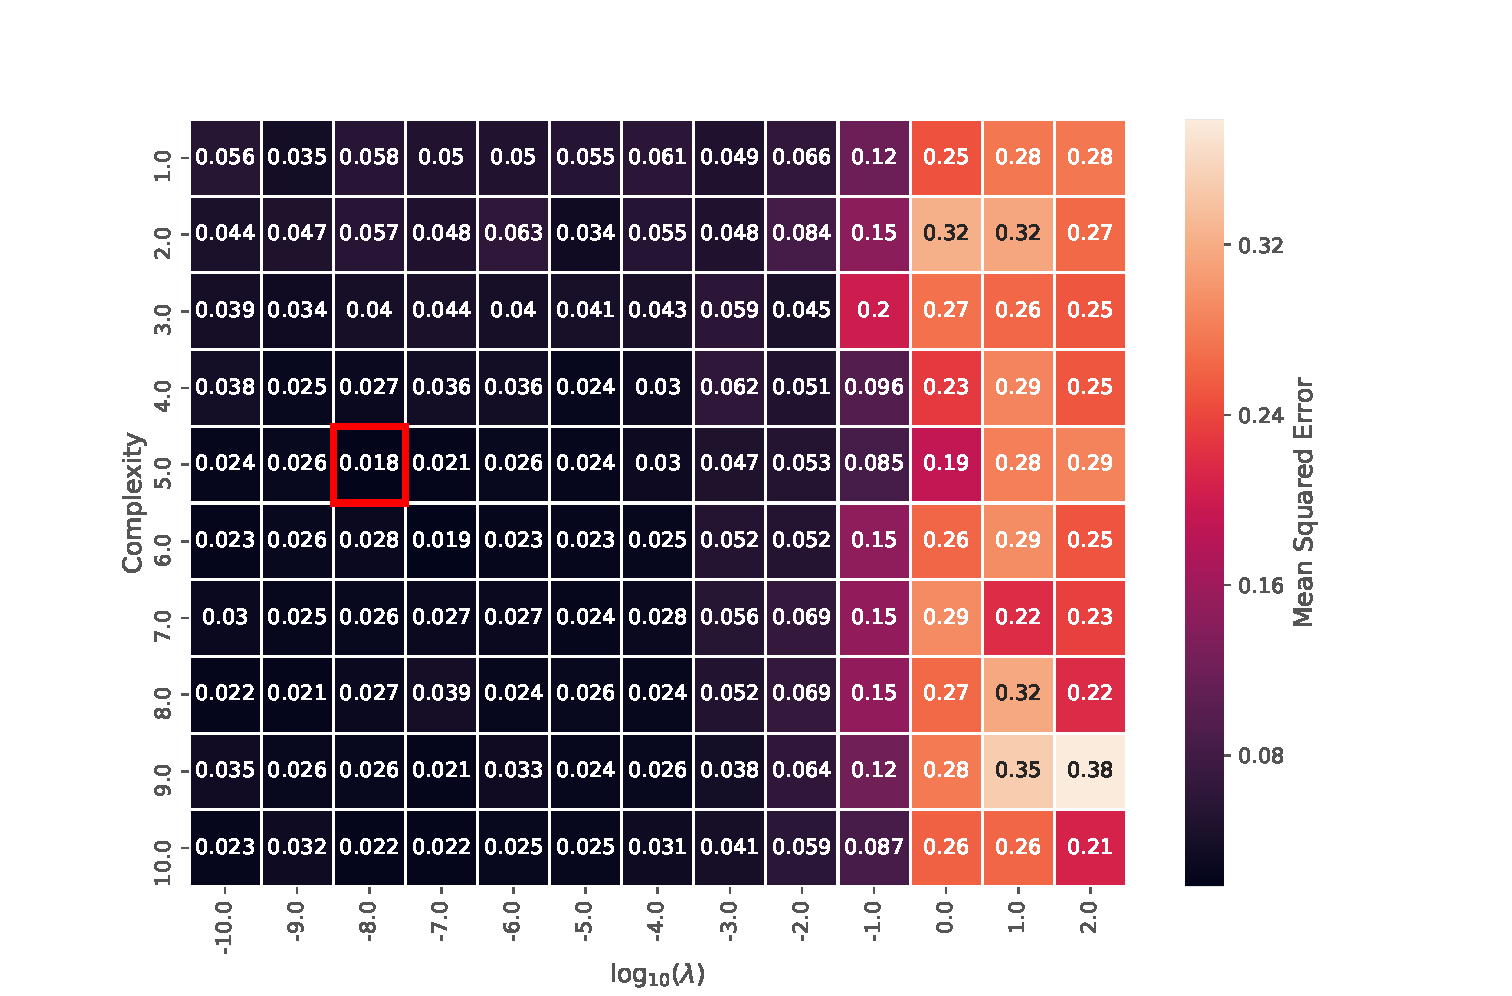
\includegraphics[scale=0.6]{Figures/LASSO/min_mse_heatmap_ridge_019.pdf}
    \caption{Heat map of the MSE of the predictions of Lasso regression on the generated data for different values of $\lambda$ and model complexity $d$. Tolerance for convergence of the gradient descent: 0.0001, maximum iterations: 10000.}
    \label{fig:lasso_heatmap}
\end{figure}

Figure \ref{fig:lasso_heatmap} shows the analysis of Lasso regression applied to the Franke function, with respect to the model complexity and the hyper parameter $\lambda$. The minimum mean squared error, $\text{MSE} = 0.0183$ was found with a polynomial degree of $d=5$ and $\lambda = 10^{-8}$, and had a corresponding $R^2$-score of $0.7874$.



\begin{figure}[!h]
    \centering
    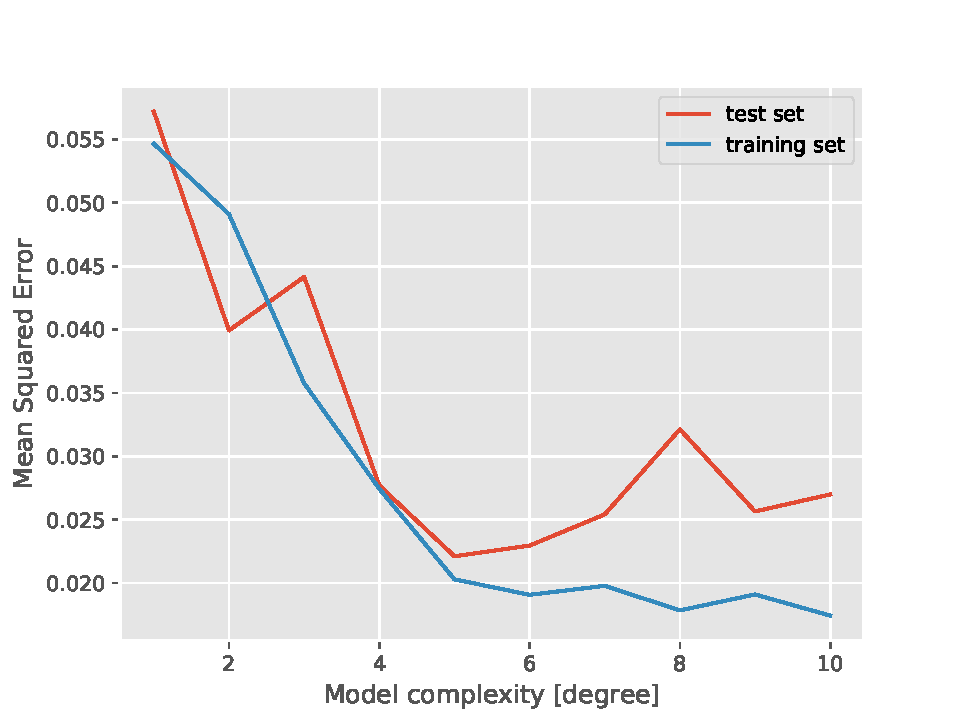
\includegraphics[scale=0.48]{Figures/LASSO/deg_analysis_lasso_test_train_020.pdf}
    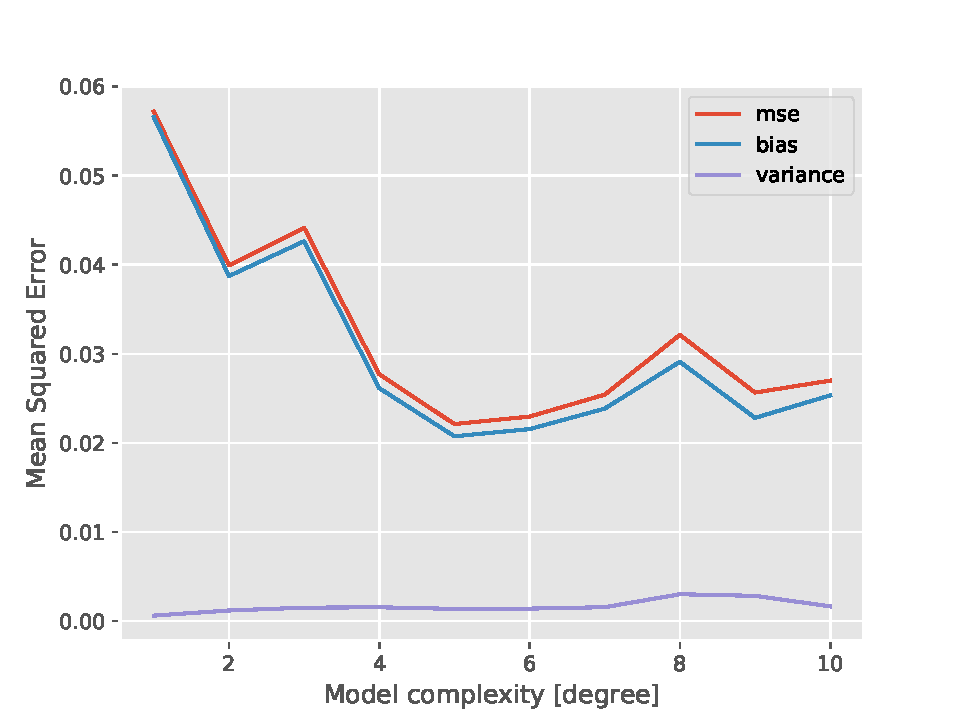
\includegraphics[scale=0.48]{Figures/LASSO/deg_analysis_lasso_bias_variance_021.pdf}
    \caption{Error in the Lasso regression prediction as a function of complexity, with $\lambda = 10^{-8}$, when modeling on the Franke data set. The left plot shows the error in the prediction on both the training and test data. The right plot shows the bias$^2$ and variance decomposition of the MSE on the test data. Tolerance for convergence of the gradient descent: 0.0001, maximum iterations: 10000.}
    \label{fig:lasso_test_train_bias_variance}
\end{figure}

In figure \ref{fig:lasso_test_train_bias_variance} we see the Lasso regression performed for different polynomial degrees, for the optimal value $\lambda=10^{-8}$. The plots shows the MSE for the training and test set, and how the MSE, bias$^2$ and variance behaves as a function of model complexity.


\begin{table}[!h]
    \caption{Comparison of the models with the lowest MSE for each regression method, applied to the Franke function data set.}
    \label{tab:franke}
    \begin{tabular}{|l|c|c|l|l|}
        \hline
        Method & degree & $\text{log}_{10} \lambda$ & MSE     & $R^2$  \\ \hline
        OLS    & 5 &  & 0.0136  & 0.819  \\ \hline
        Ridge  & 6 & -4 & 0.0139  & 0.877  \\ \hline
        Lasso  & 5 & -8 & 0.0183 & 0.728 \\ \hline
    \end{tabular}
\end{table}


\begin{figure}[!h]
    \centering
    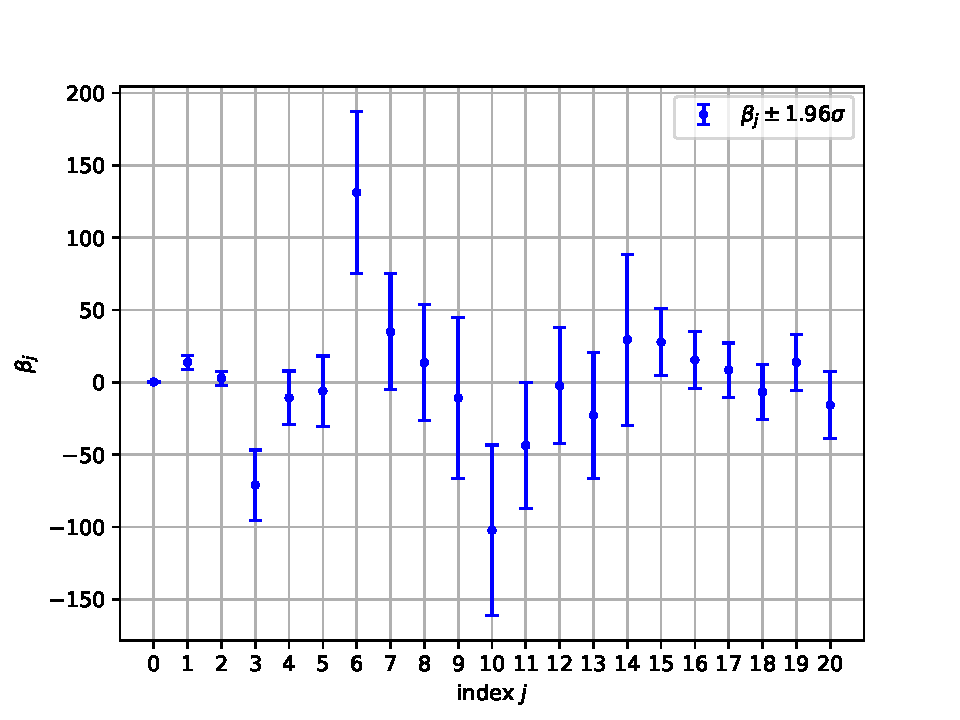
\includegraphics[scale=0.48]{Figures/OLS/confidence_interval_betas_024.pdf}
    \caption{The parameters $\beta_j$ for OLS with a confidence interval of $95\%$. Lower indices correspond to lower polynomial term coefficients, and vice verca.}
    \label{fig:ols_frankie_confidence}
\end{figure}


\subsection{Regression on real terrain data}

By doing an analysis of model complexities $d \in [1, 10]$ and hyper parameters $\log_{10}(\lambda) \in [-10, 2]$ with $100$ bootstraps, we have in table \ref{tab:terrain} listed the predicted errors of the best model configuration of the three regression methods on the real data (see section \ref{sec:data_format}). All three methods favor a polynomial of degree $d=10$, with OLS having the smallest estimate of the error, $\text{MSE} = 0.0091$. The Ridge and Lasso methods yield the best results with small values of the hyper parameter, $\lambda_{Ridge} = 10^{-9}$ and $\lambda_{Lasso} = 10^{-10}$ respectively. Figure \ref{fig:bias_variance_all_methods} shows the bias-variance decomposition of the estimated errors for the three methods for different polynomial degrees. The curve representing the MSE (the red curve) lies directly underneath the curve of the bias$^2$, and is therefore not visible in the three plots. The confidence intervals of the OLS $\beta$ parameters are shown in  \ref{fig:OLS_terrain_confidence_intervals}. In figure \ref{fig:model_terrain} we have plotted the data along side the predicted values of the OLS model with the optimal parameters found in table \ref{tab:terrain}. The appendix (sec. \ref{sec:Appendix}) contains additional plots of the results of the tuning of the $\lambda$ and $d$ parameters on the terrain data for Ridge and Lasso, as well as the error in the predictions on the test and training data for all of the three methods.

\begin{table}[!h]
    \caption{Comparison of the models with the lowest MSE for each regression method, applied to the terrain data set.}
    \label{tab:terrain}
    \begin{tabular}{|l|c|c|l|l|}
        \hline
        Method & degree & $\text{log}_{10}(\lambda)$ & MSE     & $R^2$  \\ \hline
        OLS    & 10 & - & 0.0091  & 0.6323  \\ \hline
        Ridge  & 10 & -10 & 0.0092  & 0.6325  \\ \hline
        Lasso  & 10 & -9 & 0.0138 & 0.0157 \\ \hline
    \end{tabular}
\end{table}


\begin{figure}[!h]
    \centering
    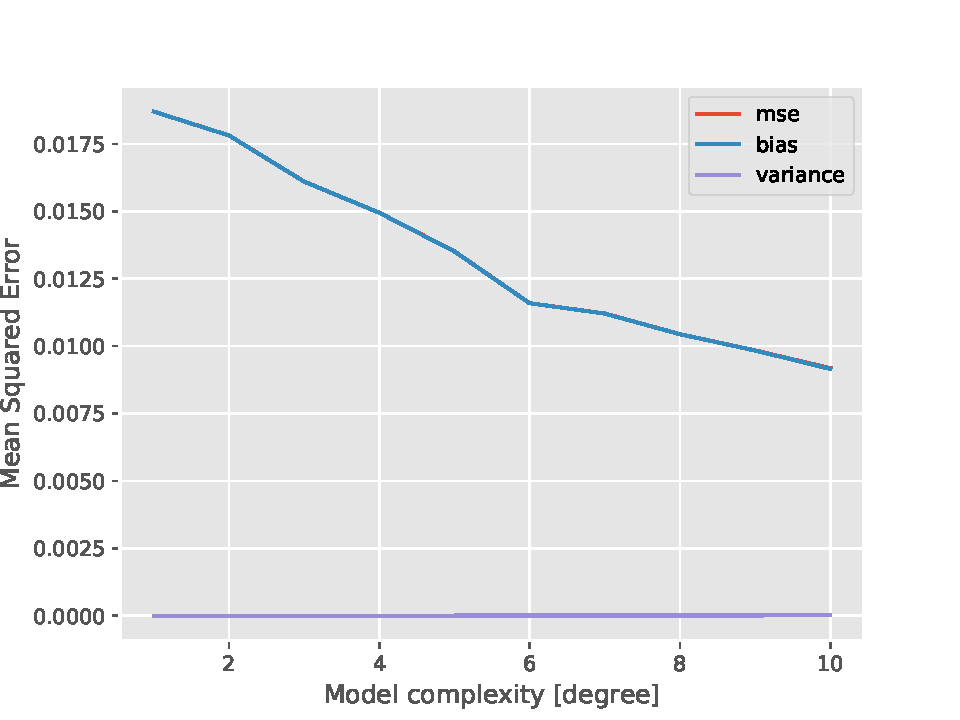
\includegraphics[scale=0.48]{Figures/RealDataPlots/deg_analysis_ols_bias_variance_016.pdf}
    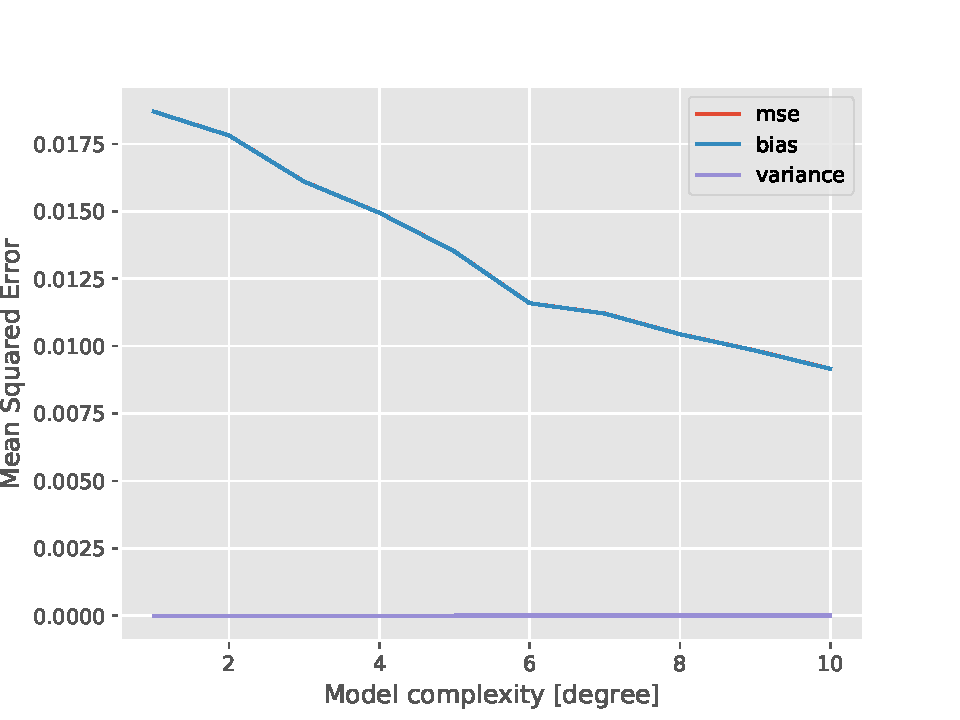
\includegraphics[scale=0.48]{Figures/RealDataPlots/deg_analysis_ridge_bias_variance_012.pdf}
    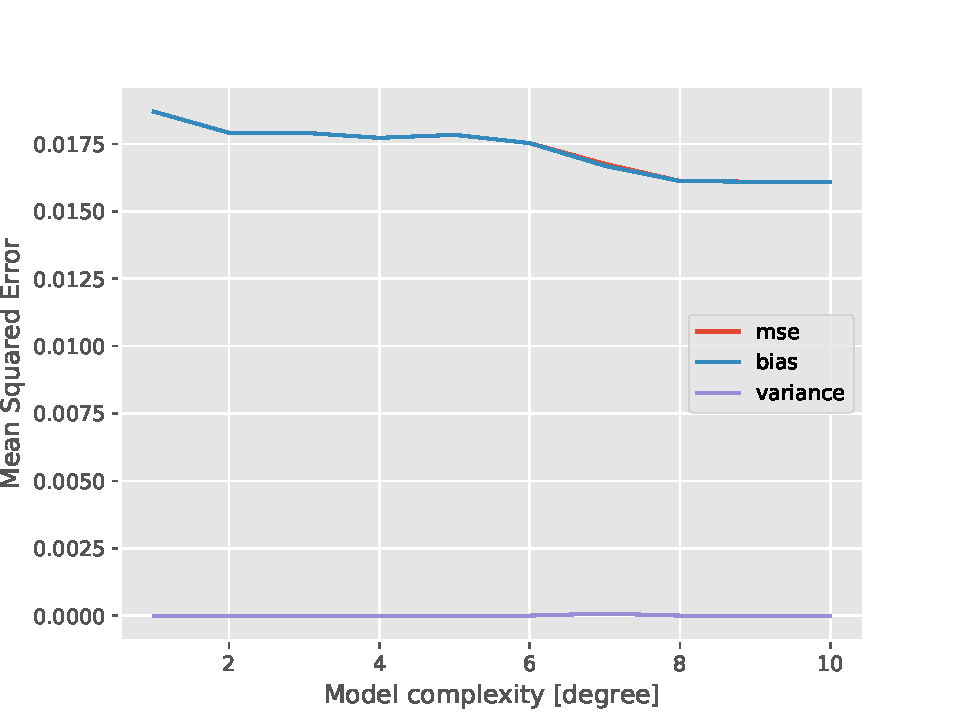
\includegraphics[scale=0.48]{Figures/RealDataPlots/deg_analysis_lasso_bias_variance_026.pdf}
    \caption{Estimated prediction errors of OLS (top left), Ridge (top right) and Lasso (bottom), and their bias$^2$ - variance decomposition as a function of model complexity.}
    \label{fig:bias_variance_all_methods}
\end{figure}

\begin{figure}[!h]
    \centering
    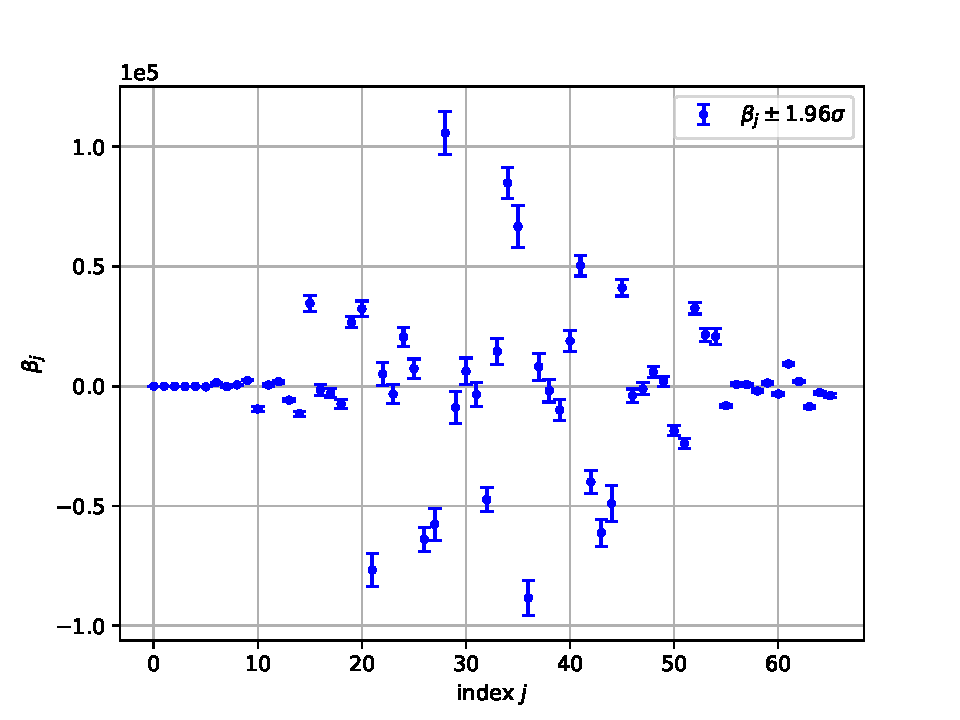
\includegraphics[scale=0.48]{Figures/RealDataPlots/confidence_interval_betas_028.pdf}
    \caption{The parameters $\beta_j$ for OLS with a confidence interval of 95\%. Lower indices correspond to lower polynomial term coefficients, and vice verca.}
    \label{fig:OLS_terrain_confidence_intervals}
\end{figure}


\begin{figure}[!h]
    \centering
    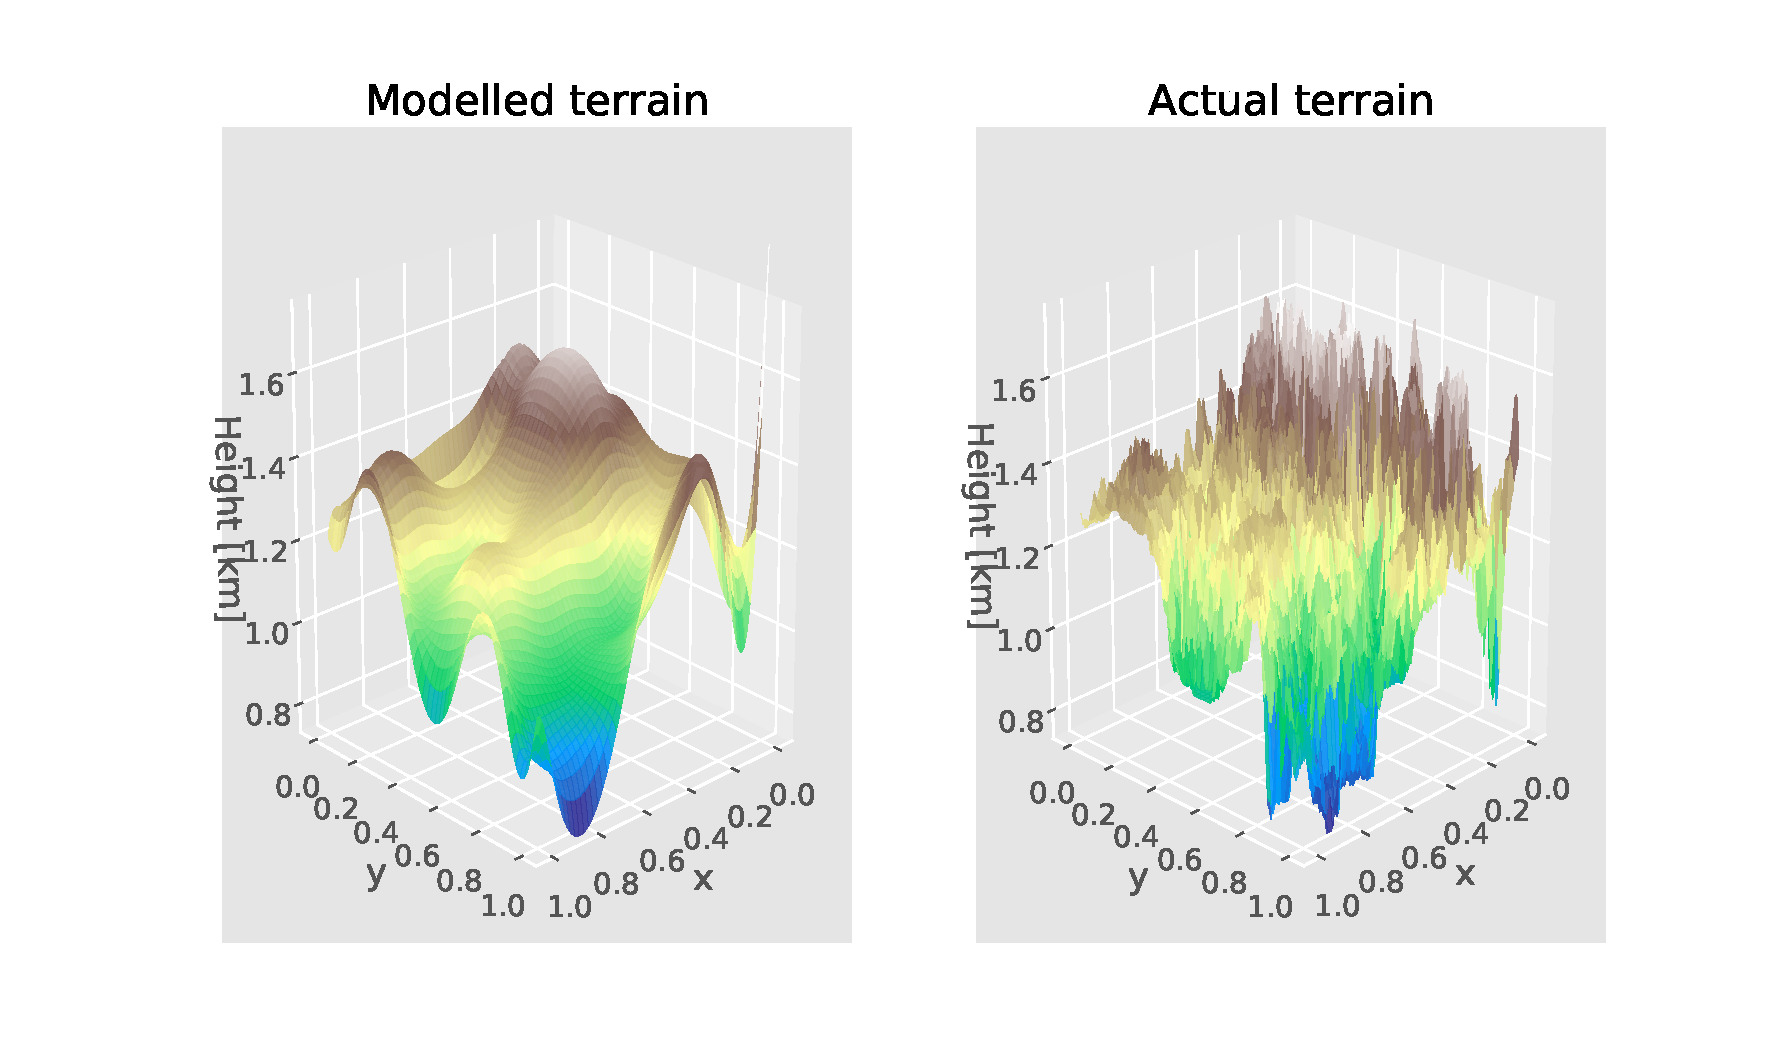
\includegraphics[scale=0.6]{Figures/RealDataPlots/model_vs_terrain_023.pdf}
    \caption{Height maps of the modelled terrain (left) and the terrain data(right).}
    \label{fig:model_terrain}
\end{figure}
\section{Discussion}\label{sec:Discussion}


\subsection{Regression on generated data}
The method of ordinary least squares gives the smallest estimation of the error, when predicting on the data generated by the Franke function. When studying the models behaviour for different complexities, we see from figure \ref{fig:ols_frankie_train_test_bias_variance} (left) that the predictions on the test set has a minimum mean squared error $\text{MSE} = 0.0136$, which occurs at degree $d = 5$. The predictions on the training set keep declining for higher complexities, while the predictions on the test set start to rise. When models of complexity $d > 5$ are introduced to data which it has not seen before, it fails to reproduce the testing data reliably. This suggests that the model has been fitted too closely to the training data and captured elements of noise, rather than the trends in the data itself.

Having a look at figure \ref{fig:ols_frankie_train_test_bias_variance} (right) again, we see that in the area $1 \leq d < 5$ the error in the prediction consists solely of the bias term, while the variance remains almost non-existent. This is most likely due to the fact that the data cannot be captured accurately by a model with such a low complexity. The predictions by the model are so off target, relatively speaking, that the differences in the training and test data are mostly irrelevant compared to the model and the trends in the data. For $d > 5$, the variance term begins increasing, while the bias declines. This is most likely due to the model being, again, over fitted, and too sensitive to small fluctuations in the data set. Ideally we want to choose a model which is complex enough to capture the regularities in the training data, but also generalized well to data which it has not seen. As seen, this middle ground is struck with a polynomial of degree $d=5$.

From \ref{tab:franke} we see that Ridge regression performs almost equally as well as OLS. With the optimal parameter $\log_{10}(\lambda) = -4$ and polynomial degree $d = 6$, the estimated error in the prediction is $\text{MSE} = 0.0139$. Having a look at the tuning of the parameters $\lambda$ and $d$ in figure \ref{fig:ridge_heatmap_frankie}, we see that its performance is generally good for small values of $\lambda$, which means that it is generally an OLS estimate, and may suggest that there is little correlation between the estimators in the model. When looking back at \ref{fig:ridge_frankie_train_test_bias_variance}, where we did a separate analysis of the performance of Ridge with the optimal value for $\lambda$, we can see that we have the same problem with overfitting when the complexity of the model is higher than $d = 6$. In this plot, the minimum MSE occurs at $d = 6$, which is different from the analysis in \ref{fig:ridge_heatmap_frankie}, even though the models had the same parameters. A possible explanation for this is the random selection of data done by the Bootstrap resampling. We have chosen a relatively small number of 100 Bootstrap resamples, which may have resulted in a fluctuation favourable to one of the configurations. In retrospect, we could have looked at the histogram of the mean values of the randomly selected values, to ensure that it was normal.

When performing Lasso regression on the generated data, we see from the heat map \ref{fig:lasso_heatmap} that the optimal model parameters which give the lowest prediction of the error $\text{MSE} = 0.0183$, are $\log_{10}(\lambda) = -8$ and complexity $d = 5$. We also see from the figure that for values of $\lambda < 1$, the model does a very bad job of reproducing the data. One reason for this may be that some of the coefficients $\beta$ have been penalized too much to be able to reproduce the data in any meaningful way. This was also true for Ridge, but even more so for Lasso, which makes sense considering that the penalization parameter in Lasso regression is capable of shrinking the $\beta$ parameters all the way to zero for greater values of $\lambda$. We have also had a closer look at the performance of the Lasso model in figure \ref{fig:lasso_test_train_bias_variance} with $\log_{10}(\lambda) = -8$, and plotted the MSE of the prediction for both the testing and training data. We see that the MSE of the test data has several local minima, which is quite interesting, and a global minimum at $d=5$ with $\text{MSE}=0.0221$. The trend of the training error keeps declining for Lasso as well, which is what we expect to see. The bias-variance decomposition of the test data error in the same figure (\ref{fig:lasso_test_train_bias_variance}) shows that the error is largely composed of the bias$^2$ term, and that the variance in the prediction is very low in comparison. In general, when comparing the Lasso method to OLS and Ridge, our results suggest that Lasso is a less suitable choice when trying to represent our data with a model. 


\subsection{Regression on real terrain data}

Figure \ref{fig:bias_variance_all_methods} shows the error analysis of the terrain data, with all three different types of regression methods. The OLS and Ridge regression gives very similar values for both the MSE, bias$^2$ and variance, which may indicate that the shrinkage imposed by the hyper parameter $\lambda$ does not contribute much to the overall result when using Ridge regression. In fact, as we can see from table \ref{tab:terrain}, the minimum MSE obtained with the OLS and Ridge method is 0.0091 and 0.0092 respectively. The OLS regression gives slightly better results, if we only use MSE as a measure of the quality of fit, but not by much. The third plot in figure \ref{fig:bias_variance_all_methods} shows the error analysis for the Lasso methods, and it shows a similar trend of the three quantities (MSE, bias$^2$ and variance) as we have seen with the OLS and Ridge regression. The minimum MSE in this case is 0.0138 for a polynomial degree $d = 10$, and clearly performs worse than the OLS and Ridge regression. All three plots show a variance that is constantly very close to zero, which means that it contributes very little to the overall error, while bias, on the other hand, is shown to be the main source of error in the models. 

Because of limitations in computational resources, we have only tested the models up to a polynomial degree of 10, but the error analysis in figure \ref{fig:bias_variance_all_methods} suggests that for all methods, the error will decrease further for higher degrees, given the declining trend of the MSE. Since our models generally have a very low variance and a relatively high bias$^2$, it seems like the models are too simple to give a good representation of the terrain.

The confidence intervals of the parameters $\beta_j$, which is presented in figure \ref{fig:OLS_terrain_confidence_intervals}, shows that the parameters with greater values generally have larger confidence intervals, which is what we would expect. The coefficients with index $j<10$ have very small values. The $\beta_j$-values with the lowest and highest indices are very small compared to the rest, and indicate that the predictors they represent do not affect the model much. As mentioned above, the bias-variance plots for the terrain model suggest that fitting with an even higher polynomial degree may have resulted in a reduced error, but in the plot of the confidence intervals of $\beta_j$ it seems like the highest order coefficients are relatively unimportant.

In figure \ref{fig:model_terrain} we see the real terrain data plotted next to our best-performing (in terms of having the lowest MSE) model, which was the OLS method with degree $d=10$. A visual inspection tells us that the model seems to be following the main features of the terrain. The edges of the surfaces are easiest to inspect, and they match fairly well. Even so, the actual topographical data is very jagged, and our model gives an oversimplified and too smooth representation of the terrain.

In all of our analysis of the methods, the models have been fitted to the training data, but since the model configurations we have found to be best in each case is based on the predictions on the test data, the reported best model configurations is by extension fitted to the test data. It may therefore be wise to in stead consider what we have called the test data in this report as validation data, and have a separate set of test data which we finally predict our ideal model on, to give a less biased estimation of the models error.
\section{Conclusion}\label{sec:Conclusion}

The aim of this project was to investigate various regression methods and resampling techniques, by testing them on two different data sets, namely generated data from the Franke function and real topographical terrain data. We tested the Ordinary Least Squares method, Ridge regression and Lasso regression, all in combination with Bootstrap resampling. Among these we obtained the lowest test error with the OLS method, on both the Franke data set and the terrain data set. When performing regression on the Franke function, the minimum MSE occured with an OLS model of polynomial degree 5, which gave $\text{MSE} = 0.0136$. Our best terrain model had $\text{MSE} = 0.0091$, when using the OLS method with polynomial degree 10. This was also the most complex model we tested for the terrain data set, and our error analysis indicated that an even higher polynomial degree might have further reduced the mean squared error.

While we could expect that the Ridge and Lasso method would reduce the error compared to the OLS method, since they in theory should lower or remove the impact of less important predictors, our analysis show that in this project the OLS model gives the best performance on test data. One reason for this might be that we failed to do an optimal normalization of our data, which may have affected both the Ridge and the Lasso regression. Also, a more fine-tuned optimalization of the hyperparameter $\lambda$ may have led to even better results. The minimum MSE-values of the Ridge regression were very close to those of OLS, and it is difficult to deem one method better than the other.

This project has shown how different types of regression methods perform on various problems, and how resampling techniques can be used to extract as much information as possible out of a data set. The error analysis we used, by observing both the mean squared error, the bias and the variance, has proven to be a very useful tool when selecting the optimal prediction model of a certain phenomenon.



%whereas Ridge regression resulted in $MSE=0.0139$ (polynomial degree 6, $\lambda=10^{-4}$ and Lasso gave $MSE=0.0183$ (polynomial degree 5, $\lambda=10^{-8}$.
 
\bibliographystyle{unsrt}
\bibliography{references}

\newpage
\section{Appendix}\label{sec:Appendix}


\begin{figure}[!h]
    \centering
    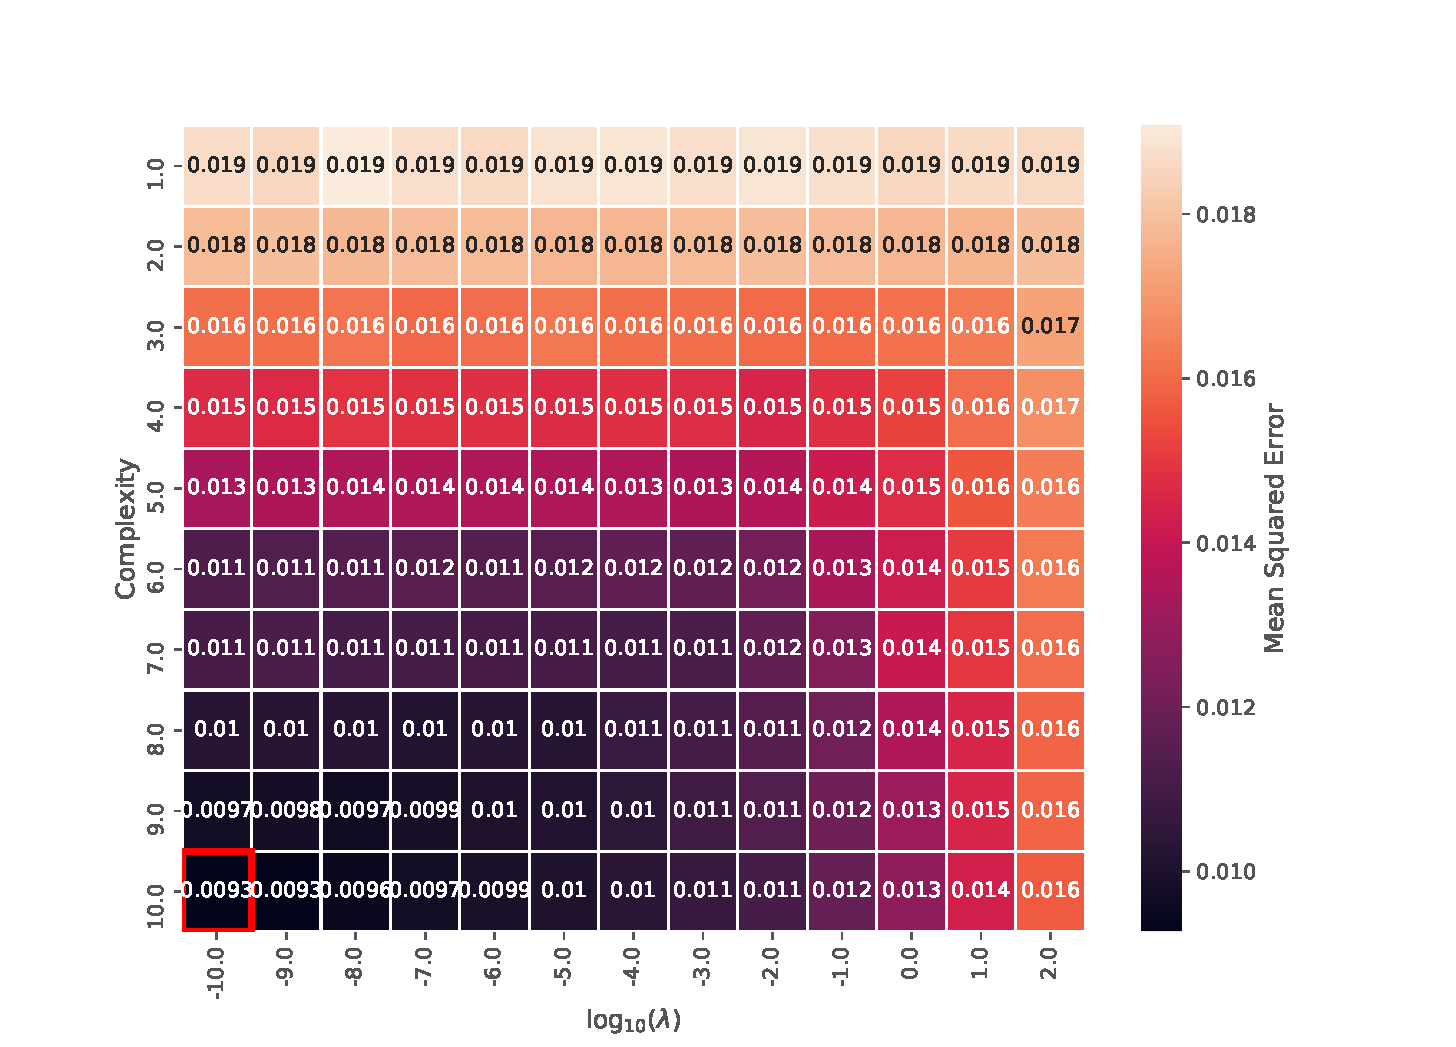
\includegraphics[scale=0.45]{Figures/APPENDIX/min_mse_heatmap_ridge_010.pdf}
    \caption{Heat map of the estimated MSE of Ridge method on the terrain data for value ranges of $\lambda$ and model complexity $d$.}
    \label{fig:appendix_heatmap_ridge}
\end{figure}

\begin{figure}[!h]
    \centering
    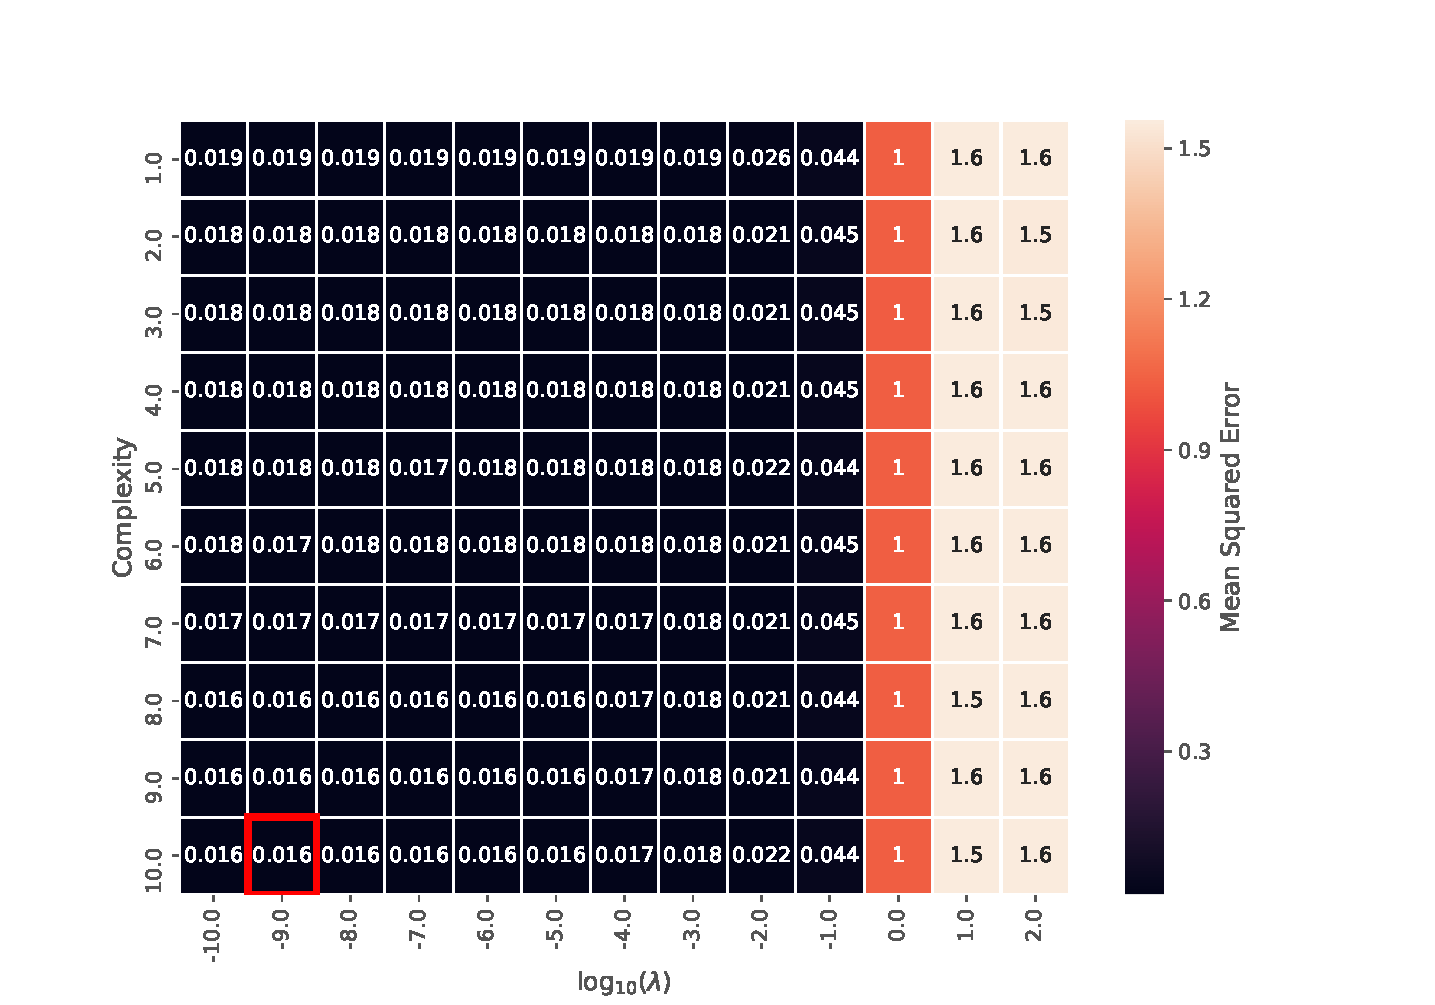
\includegraphics[scale=0.45]{Figures/APPENDIX/min_mse_heatmap_lasso_027.pdf}
    \caption{Heat map of the estimated MSE of the Lasso method on the terrain data for value ranges of $\lambda$ and model complexity $d$.}
    \label{fig:appendix_heatmap_lasso}
\end{figure}

\begin{figure}[!h]
    \centering
    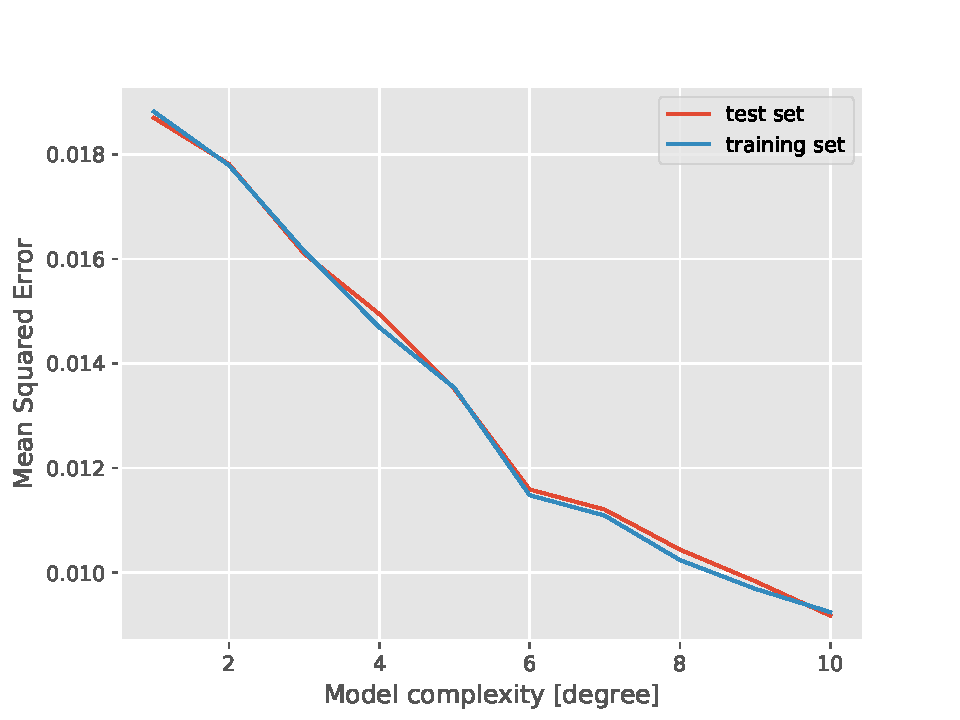
\includegraphics[scale=0.48]{Figures/APPENDIX/deg_analysis_ols_test_train_015.pdf}
    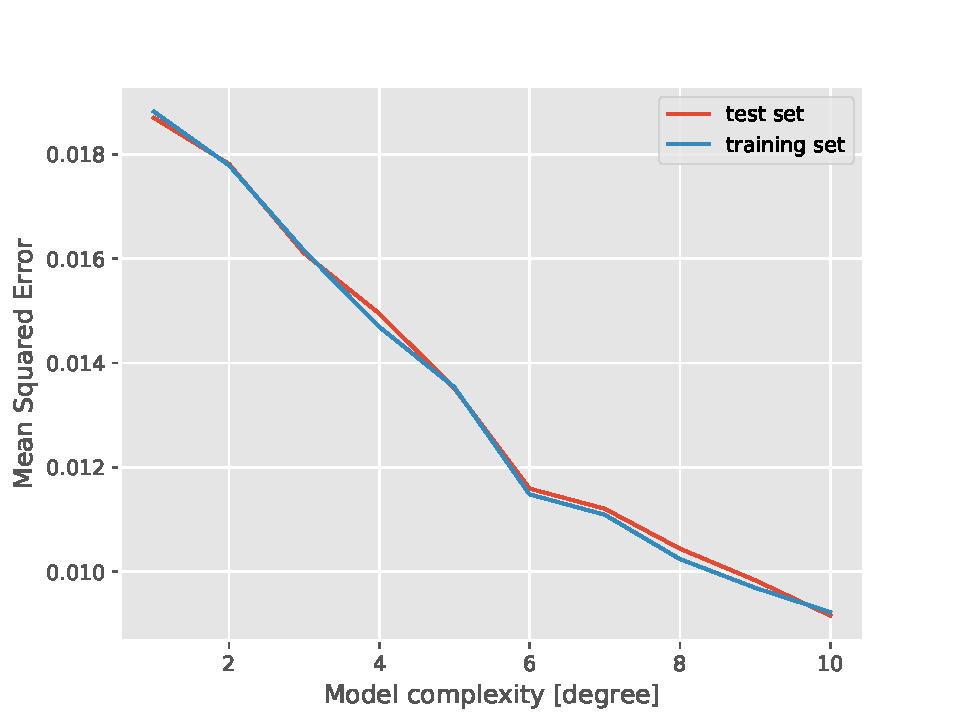
\includegraphics[scale=0.48]{Figures/APPENDIX/deg_analysis_ridge_test_train_011.pdf}
    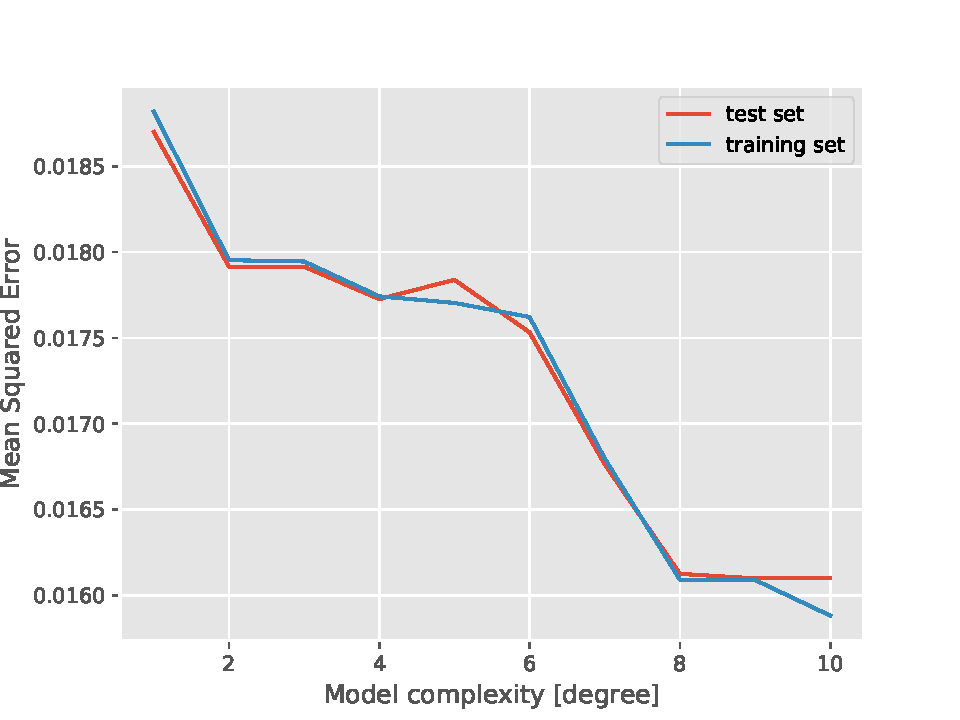
\includegraphics[scale=0.48]{Figures/APPENDIX/deg_analysis_lasso_test_train_025.pdf}
    \caption{MSE of the predictions by the OLS(top left), Ridge(top right) and Lasso(bottom) methods on the training and testing portions of the terrain data for different model complexities. $\lambda_{Ridge} = 10^{-10}$, $\lambda_{Lasso} = 10^{-9}$.}
    \label{fig:appendix_train_test}
\end{figure}


 
%\end{multicols}
\end{document}